\documentclass{scrartcl}
\input{File_Setup.tex}
\usepackage{graphicx,epsfig}
\usepackage{float}
\setcounter{topnumber}{5}
\setcounter{bottomnumber}{5}
\setcounter{totalnumber}{10} %  (for 2-column docs, often 2–3)
\renewcommand{\topfraction}{0.9}
\renewcommand{\bottomfraction}{0.9}
\renewcommand{\textfraction}{0.05}
\renewcommand{\floatpagefraction}{0.8}
\usepackage[section]{placeins}
\hypersetup{
   colorlinks   = true,
   urlcolor     = blue,
   linkcolor    = blue,
   citecolor    = red,
   setpagesize  = false,
   linktocpage  = true,
}
\graphicspath{ {fig/} }

\renewenvironment{abstract}{
    \centering
    \textbf{Abstract}
    \vspace{0.5cm}
    \par\itshape
    \begin{minipage}{0.7\linewidth}}{\end{minipage}
    \noindent\ignorespaces
}

\begin{document}
\begin{titlepage}
	\centering
	
\includegraphics[width=0.6\textwidth]{GW_logo.eps}\par
	\vspace{2cm}
	{\scshape\LARGE Data Science Program \par}
	\vspace{1cm}
	{\scshape\Large Capstone Report - Fall 2025\par}
	\vspace{1.5cm}
	{\huge\bfseries Adaptive Bandit Algorithms for Drifting Users\par}
	\vspace{2cm}
	{\Large\itshape Hema Chandra Puchakayala}\par
	\vspace{1.5cm}
	Supervised by\par
    Tyler Wallett, 
	Amir Jafari

	\vfill
	\begin{abstract}
	Modern recommender systems operate in environments where user
	preferences drift over time, breaking the stationarity assumptions of
	classical bandit algorithms. This project builds a synthetic
	drifting-user simulator and evaluates four adaptive multi-armed bandit
	methods—Non-Stationary $\varepsilon$-Greedy, Sliding-Window UCB,
	CUSUM-UCB, and EXP3.S—on their ability to track changing reward
	distributions. Each algorithm is run for 10{,}000 interaction steps
	across 50 random seeds, and performance is measured using rolling
	average and cumulative reward with confidence intervals. The results
	show that Sliding-Window UCB achieves the highest long-run reward,
	with CUSUM-UCB and Non-Stationary $\varepsilon$-Greedy forming a
	competitive middle tier, while the adversarial EXP3.S underperforms in
	this stochastic drift setting. These findings suggest that methods
	which explicitly discount or reset outdated observations are better
	suited to gradual user drift than adversarial bandit algorithms tuned
	for worst-case regret.
	\end{abstract}
	\vfill
\end{titlepage}

\tableofcontents
\newpage

% ----------------------------------------------------
\section{Introduction}

Online platforms rely on recommender systems to personalize content, ads, and
products to individual users. A central challenge in these systems is
\emph{user drift}: preferences evolve over time due to changes in taste,
context, and external trends. When rewards change independently of the system’s
actions, the problem is more naturally modeled as a non-stationary
multi-armed bandit (MAB) rather than a full Markov decision process.

This project studies how different adaptive bandit algorithms respond to user
drift in a controlled simulation environment. Users are represented by latent
preference vectors over a small set of content categories, and their
preferences follow a drifting process that gradually favors one document over
another. Within this environment, we compare four bandit strategies that have
been proposed for non-stationary or adversarial settings and quantify how well
they track the shifting reward landscape.

% ----------------------------------------------------
\section{Problem Statement}

The goal of this project is to evaluate and compare adaptive bandit algorithms
for a recommendation scenario where user preferences drift over time. We focus
on a simplified setting with two documents (arms) and a single user whose
latent preferences evolve independently of the recommender’s actions.

The main challenges are:
\begin{itemize}
	\item Designing a synthetic yet realistic drifting-user environment that
	      is reproducible across experiments.
	\item Selecting and correctly implementing bandit algorithms that embody
	      different adaptation mechanisms (sliding windows, change
	      detection, constant step-size, adversarial weighting).
	\item Defining metrics and an experimental protocol that allow a fair
	      comparison of models over long horizons and multiple random seeds.
\end{itemize}

Our objective is not to build a production-ready recommender, but to isolate
and study the adaptation behavior of these algorithms under controlled drift.

% ----------------------------------------------------
\section{Related Work}

Non-stationary bandits have been studied through a variety of approaches,
including discounted UCB, sliding-window estimators, change-detection-based
methods, and adversarial algorithms such as EXP3.\cite{swucb,epsilon_greedy_ns,
cusumucb,exp3s} Sliding-Window UCB (SW-UCB) restricts its statistics to the most
recent $\tau$ observations, allowing it to forget outdated rewards quickly.
Non-Stationary $\varepsilon$-Greedy replaces sample averages with
exponential recency-weighted estimates, providing a simple baseline for drift.

CUSUM-UCB augments the classical UCB index with a two-sided CUSUM detector
that restarts an arm when a significant mean shift is detected, making it
well-suited to piecewise-stationary environments. EXP3 and its variants, such
as EXP3.S, treat rewards as an arbitrary sequence and maintain exponential
weights over arms, mixing exploitation with uniform exploration to obtain
adversarial regret guarantees.

Our work differs from previous studies by placing these four algorithms in a
common drifting-user simulator tailored to recommender-style scenarios. The
simulator exposes a unified interface, making it straightforward to add new
algorithms and regenerate comparable results under alternative drift regimes.

% ----------------------------------------------------
\section{Solution and Methodology}

\subsection{Drifting-User Environment}

We implement a function \texttt{create\_environment} that generates a
\emph{drifting} bandit environment with $K$ arms and $T$ timesteps. At $t=0$
the user’s preference vector over arms is uniform. At each subsequent step the
vector is perturbed by Gaussian noise and renormalized to form a valid
probability distribution. This distribution is interpreted as the probability
of a click or reward for each arm, from which Bernoulli rewards are sampled.

For the experiments in this report we set $K=2$ documents and $T=10{,}000$
interaction steps. Each run is initialized with a different random seed so
that user trajectories and rewards differ across experiments while sharing the
same drift dynamics.

\subsection{Bandit Algorithms}

% ALL PREVIOUS MODELS HERE (bullet point with short description)
A wide range of strategies has been developed to address non-stationarity in
multi-armed bandit problems, particularly in settings where the reward distribution
drifts or changes abruptly over time. Classical bandit algorithms such as UCB and
$\varepsilon$-greedy assume stationary reward distributions and therefore struggle when
user preferences evolve, as their estimates place equal weight on outdated and recent
observations. To mitigate this limitation, several adaptive variants have been proposed
in the literature, each incorporating mechanisms to discount stale information, detect
distributional shifts, or explicitly reset statistics after suspected changes.

This section reviews four representative approaches that form the basis of our
comparative study: Sliding-Window UCB (SW-UCB), Non-Stationary
$\varepsilon$-Greedy, EXP3.S, and CUSUM-UCB. These methods span both stochastic
and adversarial formulations of non-stationary bandits and provide a spectrum of
adaptation mechanisms, including sliding-window averaging, exponential
recency-weighted updates, weight-sharing regularization, and online change detection.
By examining these algorithms, we establish a comprehensive foundation for evaluating 
how different adaptation strategies respond to user drift in recommendation-style 
environments.

\begin{itemize}

    % \item \textbf{LinUCB}\cite{linucb}:  
    % LinUCB is a contextual bandit algorithm that assumes a linear relationship between context features and expected rewards.  
    % For each arm $a$, LinUCB maintains an estimate of a parameter vector $\theta_a$ such that  
    % \[
    %     \mathbb{E}[r_t(a)] = x_t^\top \theta_a.
    % \]  
    % The action-selection rule uses an upper-confidence bound:  
    % \[
    %     a_t = \arg\max_a \; x_t^\top \hat{\theta}_a + \alpha \sqrt{x_t^\top A_a^{-1} x_t},
    % \]
    % where $A_a = D_a^\top D_a + I$ is the covariance matrix and $b_a = \sum r_i x_i$. The parameter estimate is  
    % \[
    %     \hat{\theta}_a = A_a^{-1} b_a. 
    % \]  
    % After observing reward $r_t$, updates are  
    % \[
    %     A_a \leftarrow A_a + x_t x_t^\top, \qquad b_a \leftarrow b_a + r_t x_t.
    % \]

    \item \textbf{Sliding-Window UCB (SW-UCB)}\cite{swucb}:  
    SW-UCB is a variant of UCB designed for non-stationary environments with abrupt changes.  
    Instead of using all past observations, it computes estimates using only the most recent $\tau$ rounds, 
    allowing rapid adaptation to changing reward distributions.  

    The sliding-window empirical mean for arm $i$ at time $t$ is  
    \[
        \bar{X}_t(\tau, i)
        = \frac{1}{N_t(\tau, i)}
        \sum_{s = t-\tau+1}^{t} X_s(i)\,\mathbbm{1}_{\{I_s = i\}},
    \]
    where  
    \[
    N_t(\gamma,i) \;=\; \sum_{s=1}^{t} \gamma^{\,t-s}\,\mathbbm{1}_{\{I_s = i\}},
    \]
 The is the number of times the arm $i$ was selected in the last $\tau$ rounds, $\gamma \in (0,1)$ is the discount factor controlling how quickly past observations are forgotten and $\xi$ is a some appropriate constant.

    SW-UCB constructs an upper-confidence bound using:  
    \[
        c_t(\tau, i)
        = B \sqrt{\frac{\xi \log (t \wedge \tau)}{N_t(\tau, i)}},
    \]
    where $B$ is the upper-bound on the rewards, $t \wedge \tau$ denotes the minimum of t and $\tau$ and $\xi > 1/2$ controls exploration.

    \textbf{Action selection is performed by}\\
\quad for $t = 1$ to $K$, play arm $I_t = t$;\\
\quad for $t = K+1$ to $T$, play arm
\[
    I_t
    = \arg\max_{1 \le i \le K}
    \left(
        \bar{X}_t(\tau,i) + c_t(\tau,i)
    \right).
\]

    After receiving the reward $X_t(a_t)$, the sliding-window statistics are updated by discarding observations older than $\tau$ rounds and inserting the new one:
    \[
        N_{t+1}(\gamma, i)
        = \sum_{s = t-\tau+2}^{t+1} \gamma^{\,t+1-s}\, \mathbbm{1}_{\{I_s = i\}},
    \]
    \[
        \bar{X}_{t+1}(\tau, a)
        = \frac{1}{N_{t+1}(\tau, a)}
          \sum_{s = t-\tau+2}^{t+1} X_s(i)\,\mathbbm{1}_{\{I_s = i\}},
    \]
    \[
        c_{t+1}(\tau, i)
        = B \sqrt{\frac{\xi \log((t+1) \wedge \tau)}{N_{t+1}(\tau, i)}}.
    \]

    \item \textbf{Non-Stationary Epsilon-Greedy}\cite{epsilon_greedy_ns}: 
    This is an adaptation of the classical $\varepsilon$-greedy method for
    environments in which the reward distributions drift over time.  
    Instead of sample averages, the action-value estimates use a
    \emph{constant step-size} update, which implements an
    exponential recency-weighted average that discounts older rewards.

    The estimate of the value of arm $i$ at time $t$ is updated according to
    the incremental constant–step-size rule  
    \[
        Q_{t+1}(i)
        \;=\;
        Q_t(i)
        \;+\;
        \alpha\Big(R_t - Q_t(i)\Big)\,\mathbbm{1}_{\{I_t = i\}},
    \]
    where $\alpha \in (0,1]$ is the constant step-size parameter.  
    Unrolling this recursion gives the exponential recency-weighted form
    \[
        Q_{t+1}(i)
        \;=\;
        (1-\alpha)^{t} Q_1(i)
        \;+\;
        \sum_{s=1}^{t}
        \alpha(1-\alpha)^{t-s}\,R_s\,\mathbbm{1}_{\{I_s=i\}},
    \]
    showing that recent rewards receive more weight than older ones, with
    decay factor $(1-\alpha)$.

    \textbf{Action selection is performed using} the $\varepsilon$-greedy policy:\\
\quad for $t = 1$ to $K$, play arm $I_t = t$;\\
\quad for $t = K+1$ to $T$, select arm
    \[
        I_t
        =
        \begin{cases}
            \text{a random arm in }\{1,\dots,K\}, & \text{with probability }\varepsilon, \\[6pt]
            \displaystyle \arg\max_{1\le i\le K} Q_t(i),     & \text{with probability }1-\varepsilon.
        \end{cases}
    \]

    After observing reward $R_t$, the value estimates are updated using the
    constant step-size rule:
    \[
        Q_{t+1}(I_t)
        =
        Q_t(I_t)
        +
        \alpha\,\big(R_t - Q_t(I_t)\big).
    \]

    Because the estimate $Q_t(i)$ places exponentially decaying weight on past
    rewards with weights proportional to $(1-\alpha)^k$ for $k$-step-old
    observations method adapts effectively to non-stationary reward
    distributions. Larger values of $\alpha$ allow faster adaptation, while
    smaller values provide greater stability.

    \item \textbf{EXP3.S}\cite{exp3s}:  
EXP3.S is a variant of the EXP3 algorithm proposed in Auer et al. (1995) \cite{exp3} designed to control regret against \emph{arbitrary} (possibly switching) action sequences.
Rather than competing only with the best single arm, EXP3.S adapts to
piecewise-stationary environments by incorporating an additional
stabilization term in the weight update that helps the algorithm track
changing optimal arms.

Like EXP3, it maintains exponential weights over the $K$ arms and mixes
between exploitation and uniform exploration.  
However, EXP3.S adds a regularization term proportional to 
$\alpha$ that penalizes rapid fluctuations and allows regret bounds
scaling with the \emph{hardness} of the comparator sequence (i.e., the number of switches throughout the sequence).

\vspace{4pt}
\textbf{Action selection:}\\
\quad At each round $t$, compute the probability distribution
\[
    p_i(t)
    \;=\;
    (1-\gamma)\,
    \frac{w_i(t)}{\sum_{j=1}^K w_j(t)}
    \;+\;
    \frac{\gamma}{K},
    \qquad i=1,\dots,K.
\]
\quad Then draw action $I_t$ according to the distribution $p(t)$.

\vspace{4pt}
\textbf{Reward estimation:}\\
After receiving reward $x_{I_t}(t) \in [0,1]$, define the unbiased
importance-weighted estimator
\[
    \widehat{x}_j(t)
    \;=\;
    \begin{cases}
        \displaystyle \frac{x_j(t)}{p_j(t)}, & j = I_t,\\[6pt]
        0, & j \neq I_t .
    \end{cases}
\]

\vspace{4pt}
\textbf{Weight update:}\\
For each arm $j = 1,\dots,K$, update
\[
    w_j(t+1)
    \;=\;
    w_j(t)\,
    \exp\!\left(\frac{\gamma}{K}\,\widehat{x}_j(t)\right)
    \;+\;
    \frac{e{\alpha}}{K}
    \sum_{i=1}^K w_i(t).
\]

The additive term
\[
    \frac{e{\alpha}}{K}\sum_{i=1}^K w_i(t)
\]
helps the algorithm adapt to environments where the best arm switches,
enabling regret bounds that depend on the number of switches rather than on~$T$ alone.


\item \textbf{CUSUM-UCB}\cite{cusumucb}:
CUSUM-UCB is a change–detection based bandit algorithm designed for
piecewise-stationary environments. It augments the classical UCB index
with a two-sided online CUSUM detector that monitors each arm for
statistically significant shifts in its reward distribution. When a
change is detected on arm $i$, the algorithm \emph{restarts} that arm by
resetting its empirical mean, sample count, and the associated CUSUM
statistics. This prevents outdated pre-change rewards from contaminating
the UCB estimate and enables rapid recovery after abrupt changes.
For each arm, the first $M$ observations are used to estimate the
pre-change mean,
\[
\hat u_0 \;=\; \frac{1}{M}\sum_{k=1}^{M} y_k,
\]
and for each subsequent sample $y_k$, the CUSUM updates use the steps
\[
(s_k^+, s_k^-) \;=\; (y_k - \hat u_0 - \varepsilon,\;\; \hat u_0 - y_k - \varepsilon)\,\mathbbm{1}_{\{k > M\}},
\]
\[
g_k^+ = \max\{0,\; g_{k-1}^+ + s_k^+\}, \qquad 
g_k^- = \max\{0,\; g_{k-1}^- + s_k^-\}.
\]
A change is detected whenever either statistic crosses the threshold $h$,
i.e.,
\[
g_k^+ \ge h \quad \text{or} \quad g_k^- \ge h,
\]
upon which the corresponding arm is restarted:
its restart time $\tau_i$ is set to the current round, and the CUSUM
variables $(g_k^+, g_k^-)$ are reset to zero.

The UCB part of the algorithm uses only post-restart statistics.
Let $\tau_i$ denote the last restart time of arm $i$. Then its valid
sample count, empirical mean, and confidence padding at time $t$ are
\[
N_t(i) = \sum_{s=\tau_i}^{t} \mathbbm{1}_{\{I_s = i\}}, \qquad
\bar X_t(i) = \frac{1}{N_t(i)}\sum_{s=\tau_i}^{t} X_s(i)\,\mathbbm{1}_{\{I_s = i\}},
\]
\[
C_t(i) = \sqrt{\frac{\xi \log n_t}{N_t(i)}}, \qquad
n_t = \sum_{j=1}^{K} N_t(j),
\]
where $\xi > 0$ is the UCB exploration constant.

\textbf{Action selection} combines UCB exploitation with uniform
sampling at rate $\alpha$, as required to feed the CUSUM detectors:
\[
I_t = 
\begin{cases}
\displaystyle \arg\max_{1\le i\le K}\bigl(\bar X_t(i) + C_t(i)\bigr), & \text{with probability } 1 - \alpha,\\[8pt]
\text{a uniformly random arm in }\{1,\dots,K\}, & \text{with probability } \alpha/K.
\end{cases}
\]

\textbf{Update rule:}
After observing reward $X_t(I_t)$, the algorithm
\begin{enumerate}
\item updates the CUSUM statistics $g_k^+,g_k^-,s_k^+,s_k^-$ for the played arm;
\item if a CUSUM alarm is raised, resets $\tau_{I_t}=t+1$ and clears the CUSUM state;
\item otherwise, updates $(N_t(i),\bar X_t(i),C_t(i))$ for the played arm using the post-restart definitions above.
\end{enumerate}
Because all pre-change samples of an arm are discarded upon detection,
CUSUM-UCB avoids the slow recovery faced by classical UCB when reward
means abruptly decrease. 
\end{itemize}

   




All algorithms are implemented in a common interface with \texttt{train}
methods that accept a matrix of rewards and return per-step reward sequences
and arm selections for analysis.

\subsection{Experimental Protocol}

For each algorithm we run 50 independent experiments with distinct seeds. In
every run, the environment first generates a full $T \times K$ reward matrix
from the drifting-user process. The algorithm then interacts with this matrix
for $T$ steps, observing one reward per round and updating its internal state.
\FloatBarrier 
We log:
\begin{itemize}
	\item The realized reward $R_t$ at each step.
	\item A one-hot encoded action vector indicating the selected arm.
\end{itemize}
For each model and metric we then average over the 50 runs and compute
pointwise $95\%$ confidence intervals based on the empirical standard error.

% ----------------------------------------------------
\section{Results and Discussion}

\subsection{Experimentation Protocol}

The main evaluation metrics are:
\begin{itemize}
	\item \emph{Rolling average reward}
	\[
	\bar{R}(t) = \frac{1}{t}\sum_{s=1}^{t} R_s,
	\]
	which reflects adaptation speed and stability over time.
	\item \emph{Cumulative reward}
	\[
	R_{\mathrm{cum}}(T) = \sum_{t=1}^{T} R_t,
	\]
	which captures total utility over the horizon.
\end{itemize}
Both metrics are reported as mean curves with $95\%$ confidence bands over 50
runs. The best model is identified as the algorithm with the highest final
cumulative reward $R_{\mathrm{cum}}(T)$, while overlapping confidence intervals
are used to judge whether differences are practically meaningful.

\subsection{Graphs}

Figure~\ref{fig:env-arms} illustrates the average and cumulative reward of each
arm in the drifting environment, aggregated over all runs. Initially both arms
are symmetric, but as the user’s latent preferences drift, one arm becomes
consistently more rewarding. The widening gap between curves shows that the
environment poses a genuine tracking challenge for bandit algorithms.

\begin{figure}[!htbp]
	\centering
	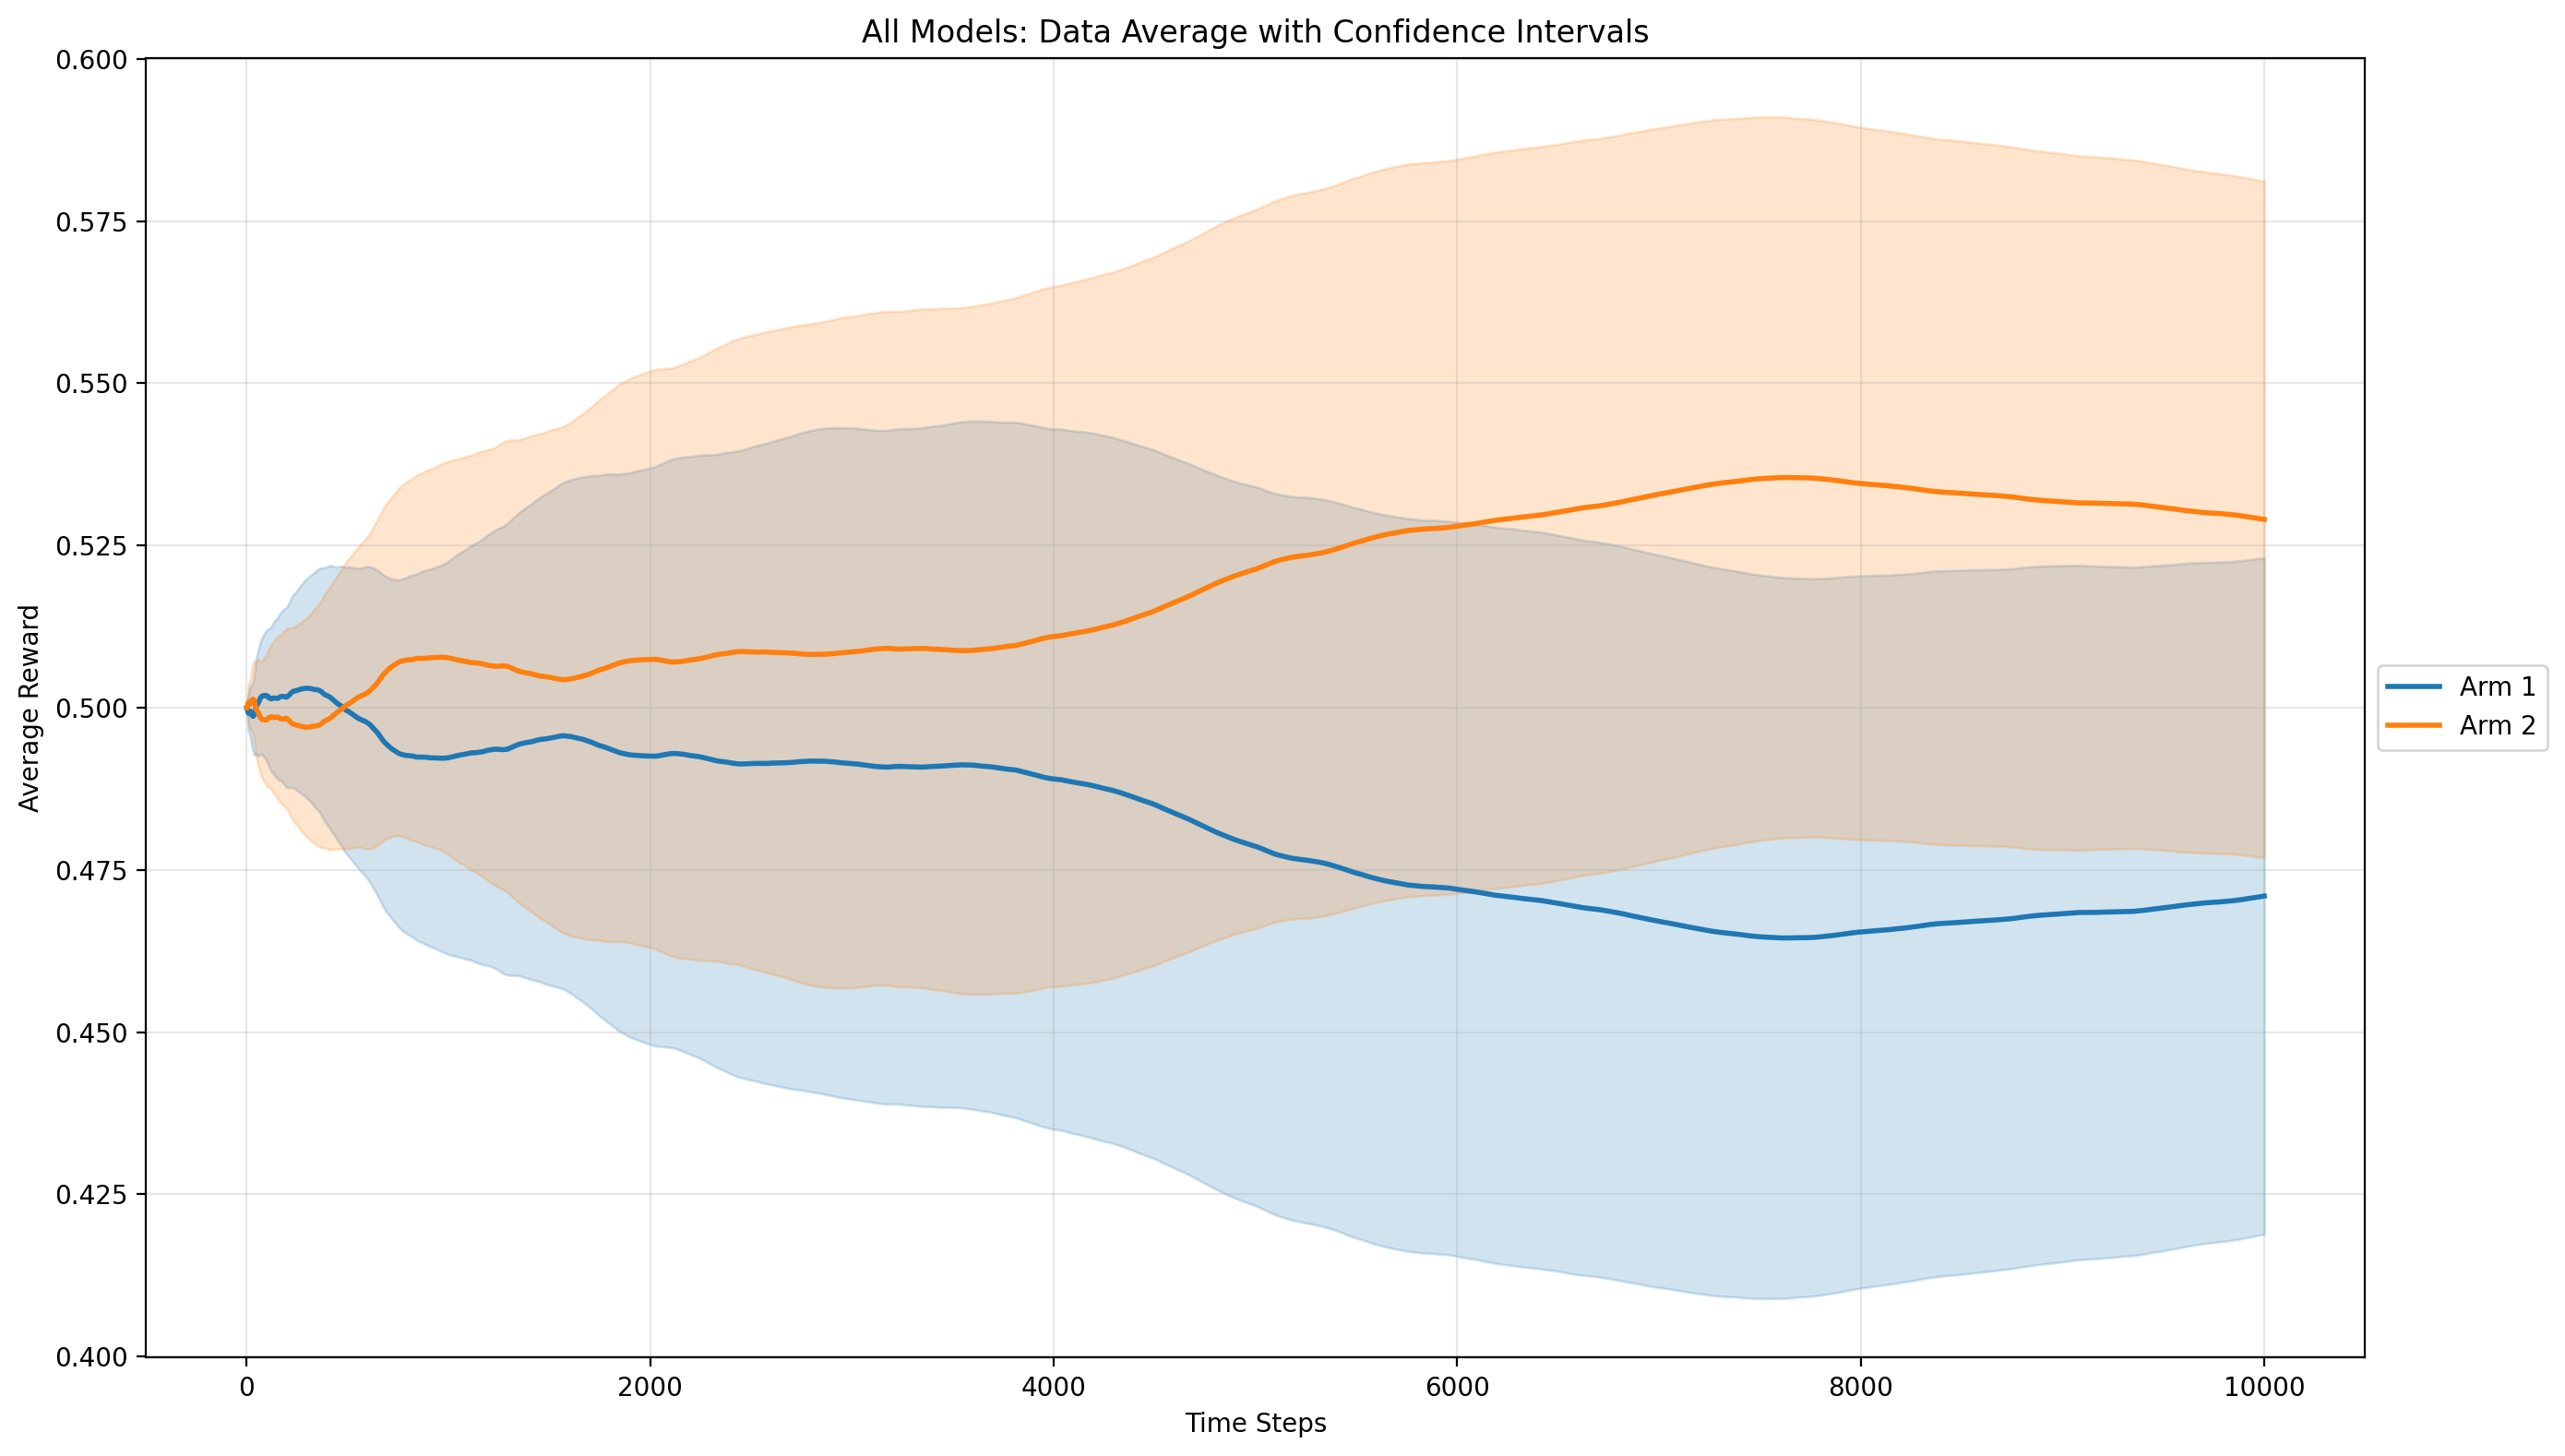
\includegraphics[width=0.9\linewidth]{all_models_average_ci.png}\\[0.5em]
	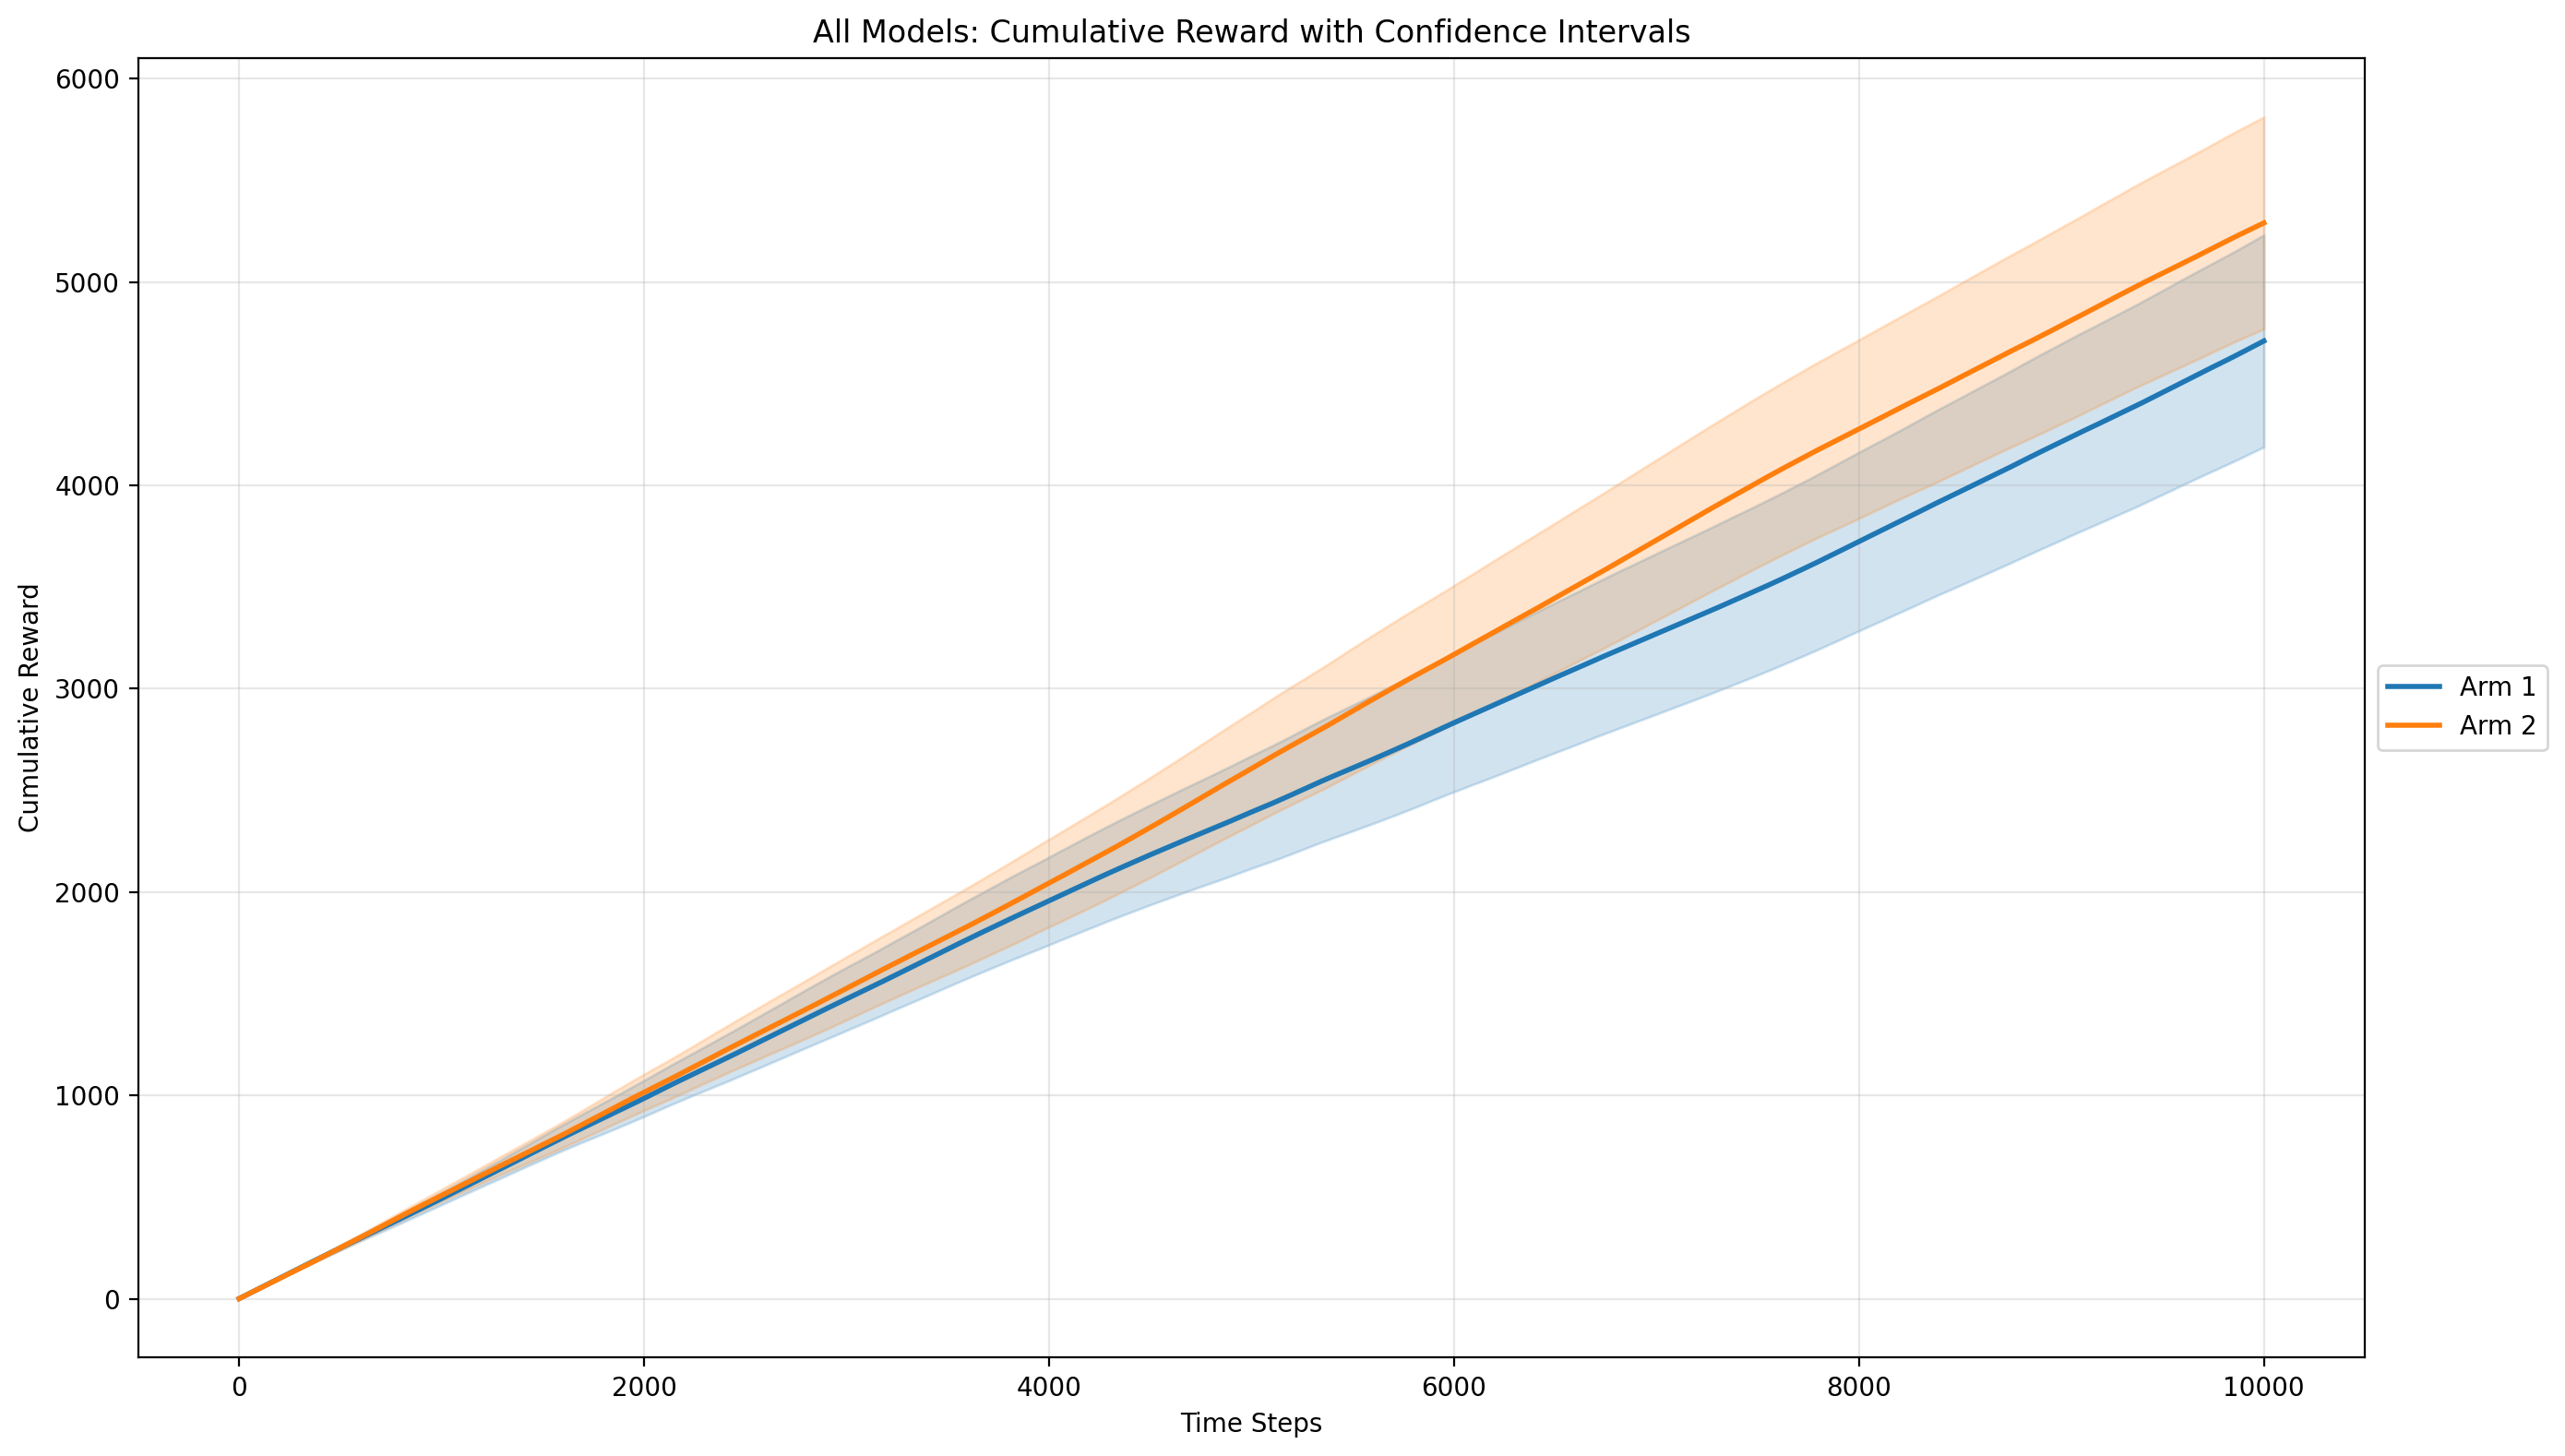
\includegraphics[width=0.9\linewidth]{all_models_cumulative_ci.png}
	\caption{Drifting-user environment: rolling average (top) and cumulative
	reward (bottom) for each arm, averaged over 50 runs with 95\% confidence
	intervals.}
	\label{fig:env-arms}
\end{figure}

Figure~\ref{fig:models-perf} compares the four algorithms. The top panel shows
the rolling average reward; the bottom panel shows cumulative reward. All
stochastic bandits improve quickly from the initial $0.5$ baseline, but
Sliding-Window UCB rises fastest and stabilizes at the highest average reward.
CUSUM-UCB and Non-Stationary $\varepsilon$-Greedy plateau at slightly lower
levels, whereas EXP3.S increases slowly and remains substantially below the
others throughout the horizon.

\begin{figure}[!htbp]
	\centering
	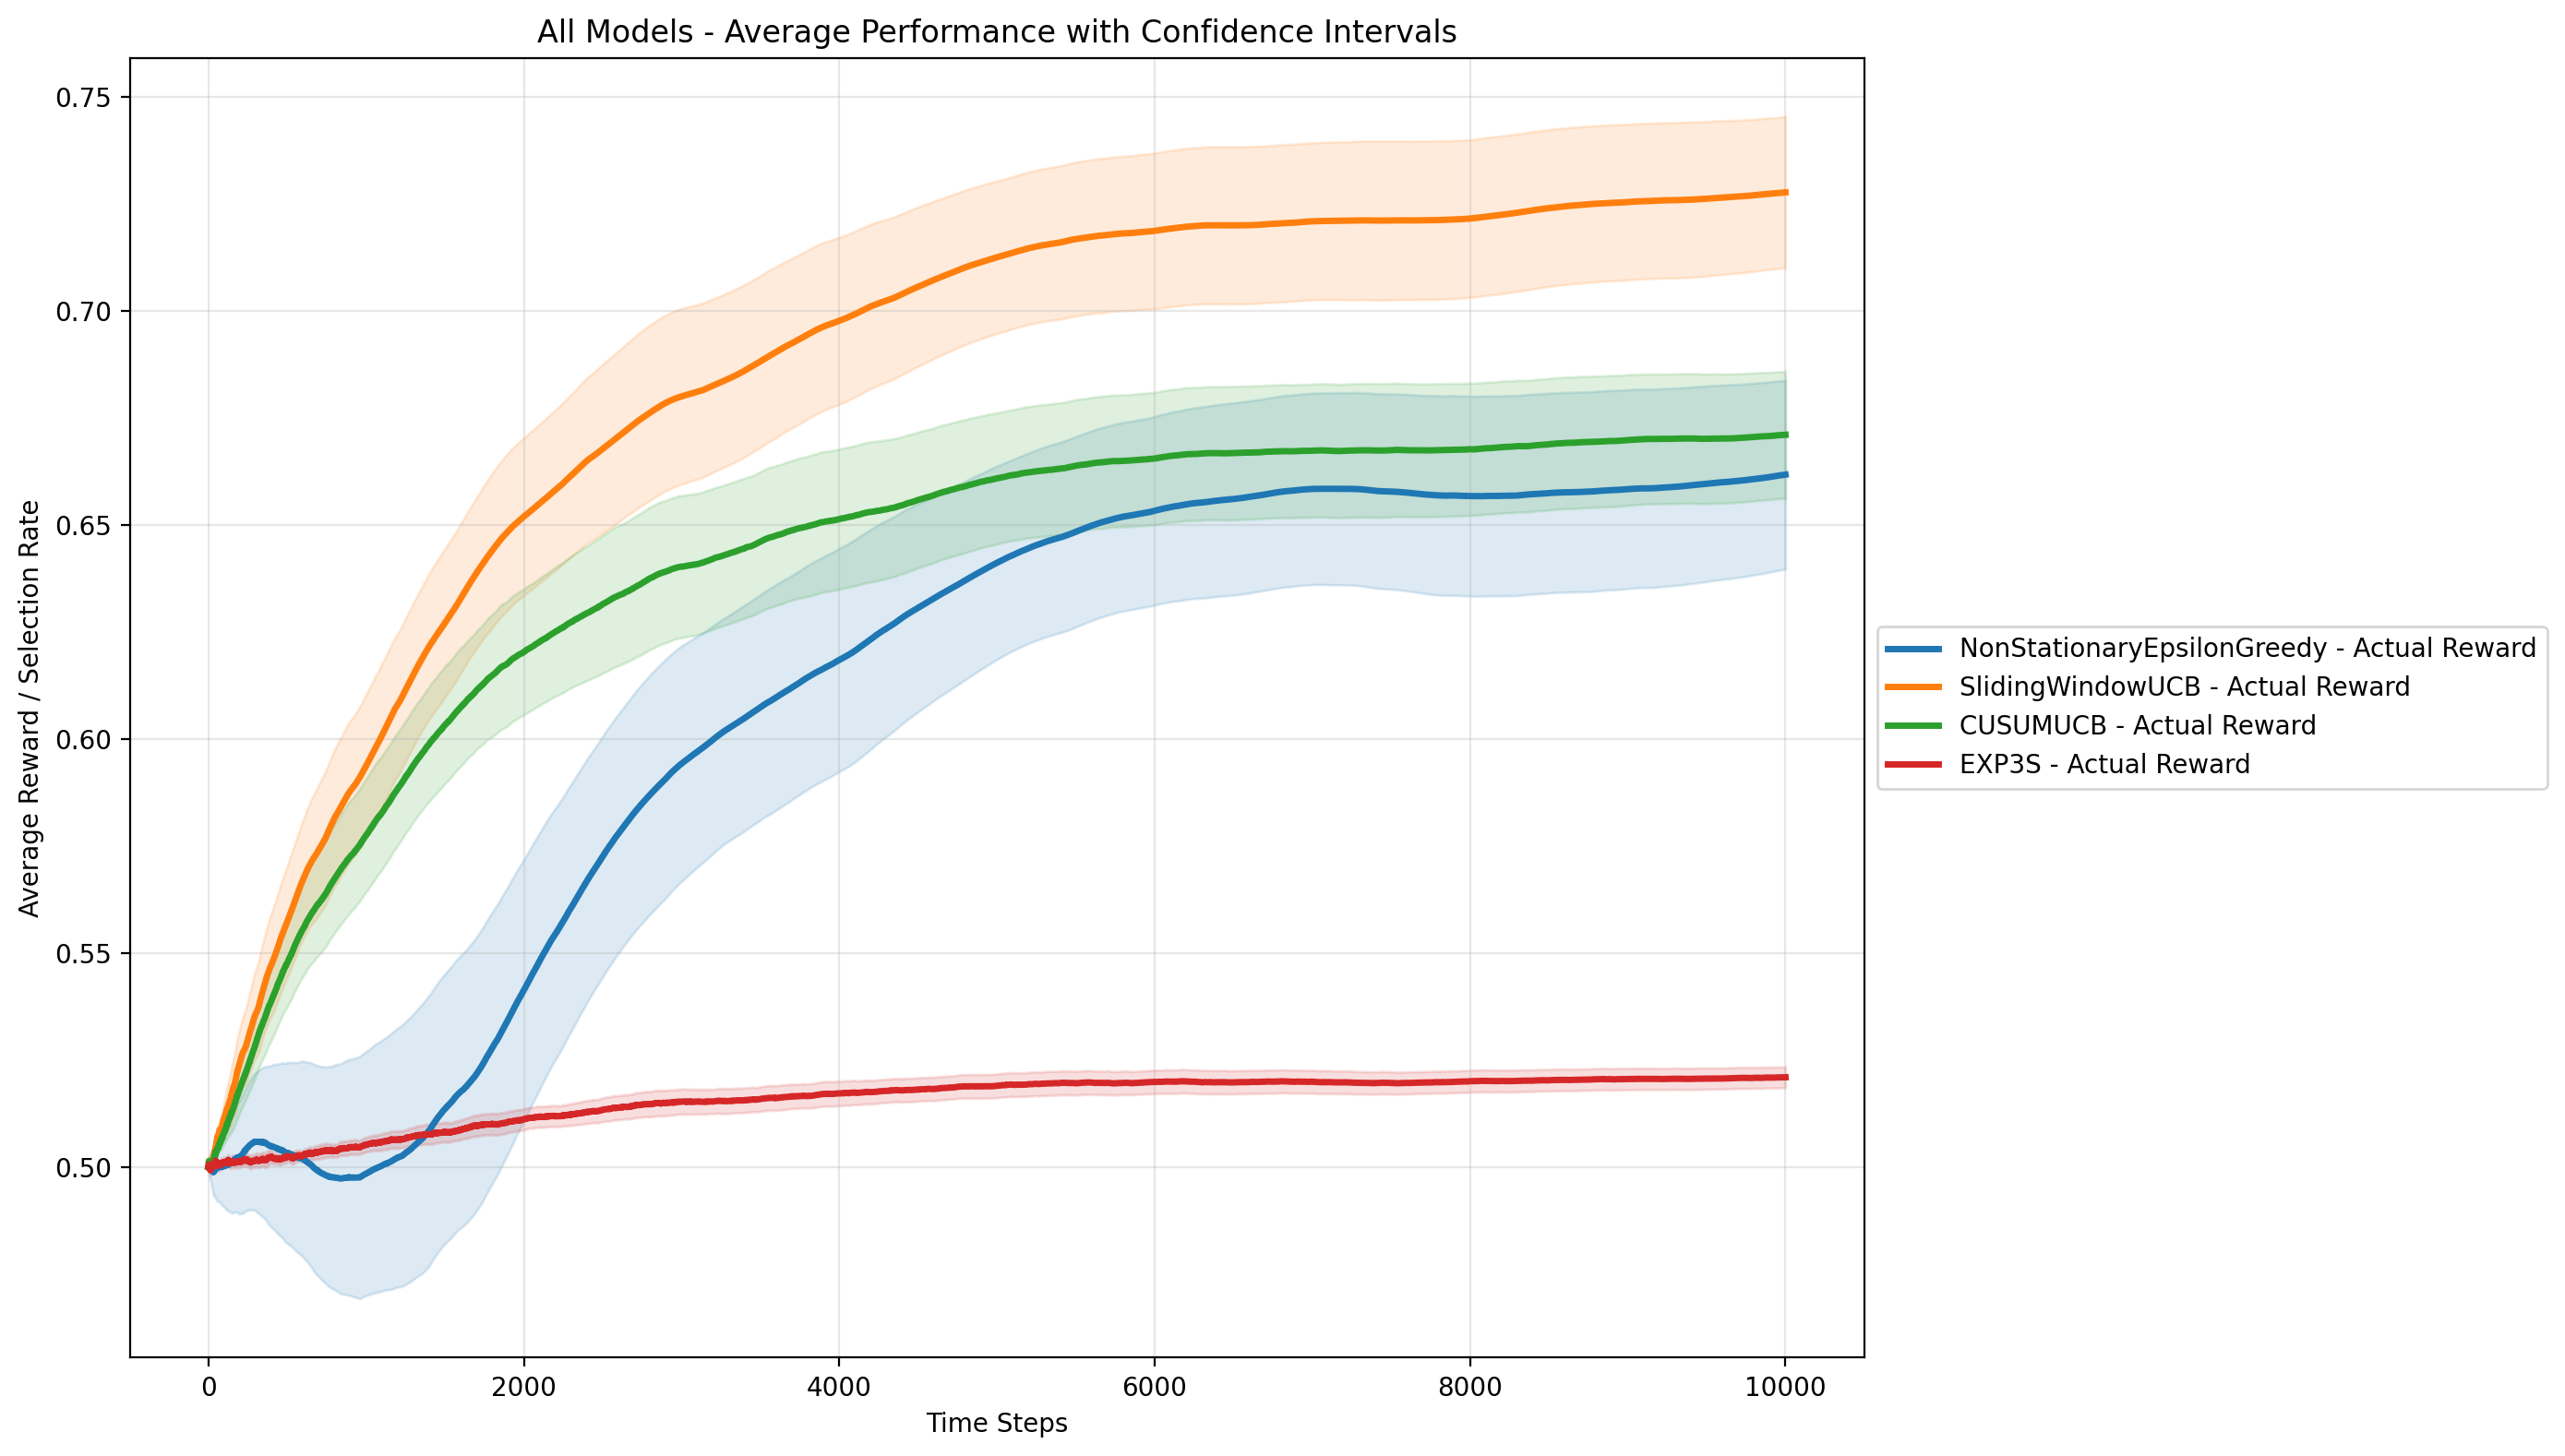
\includegraphics[width=0.9\linewidth]{model_average_all_ci.png}\\[0.5em]
	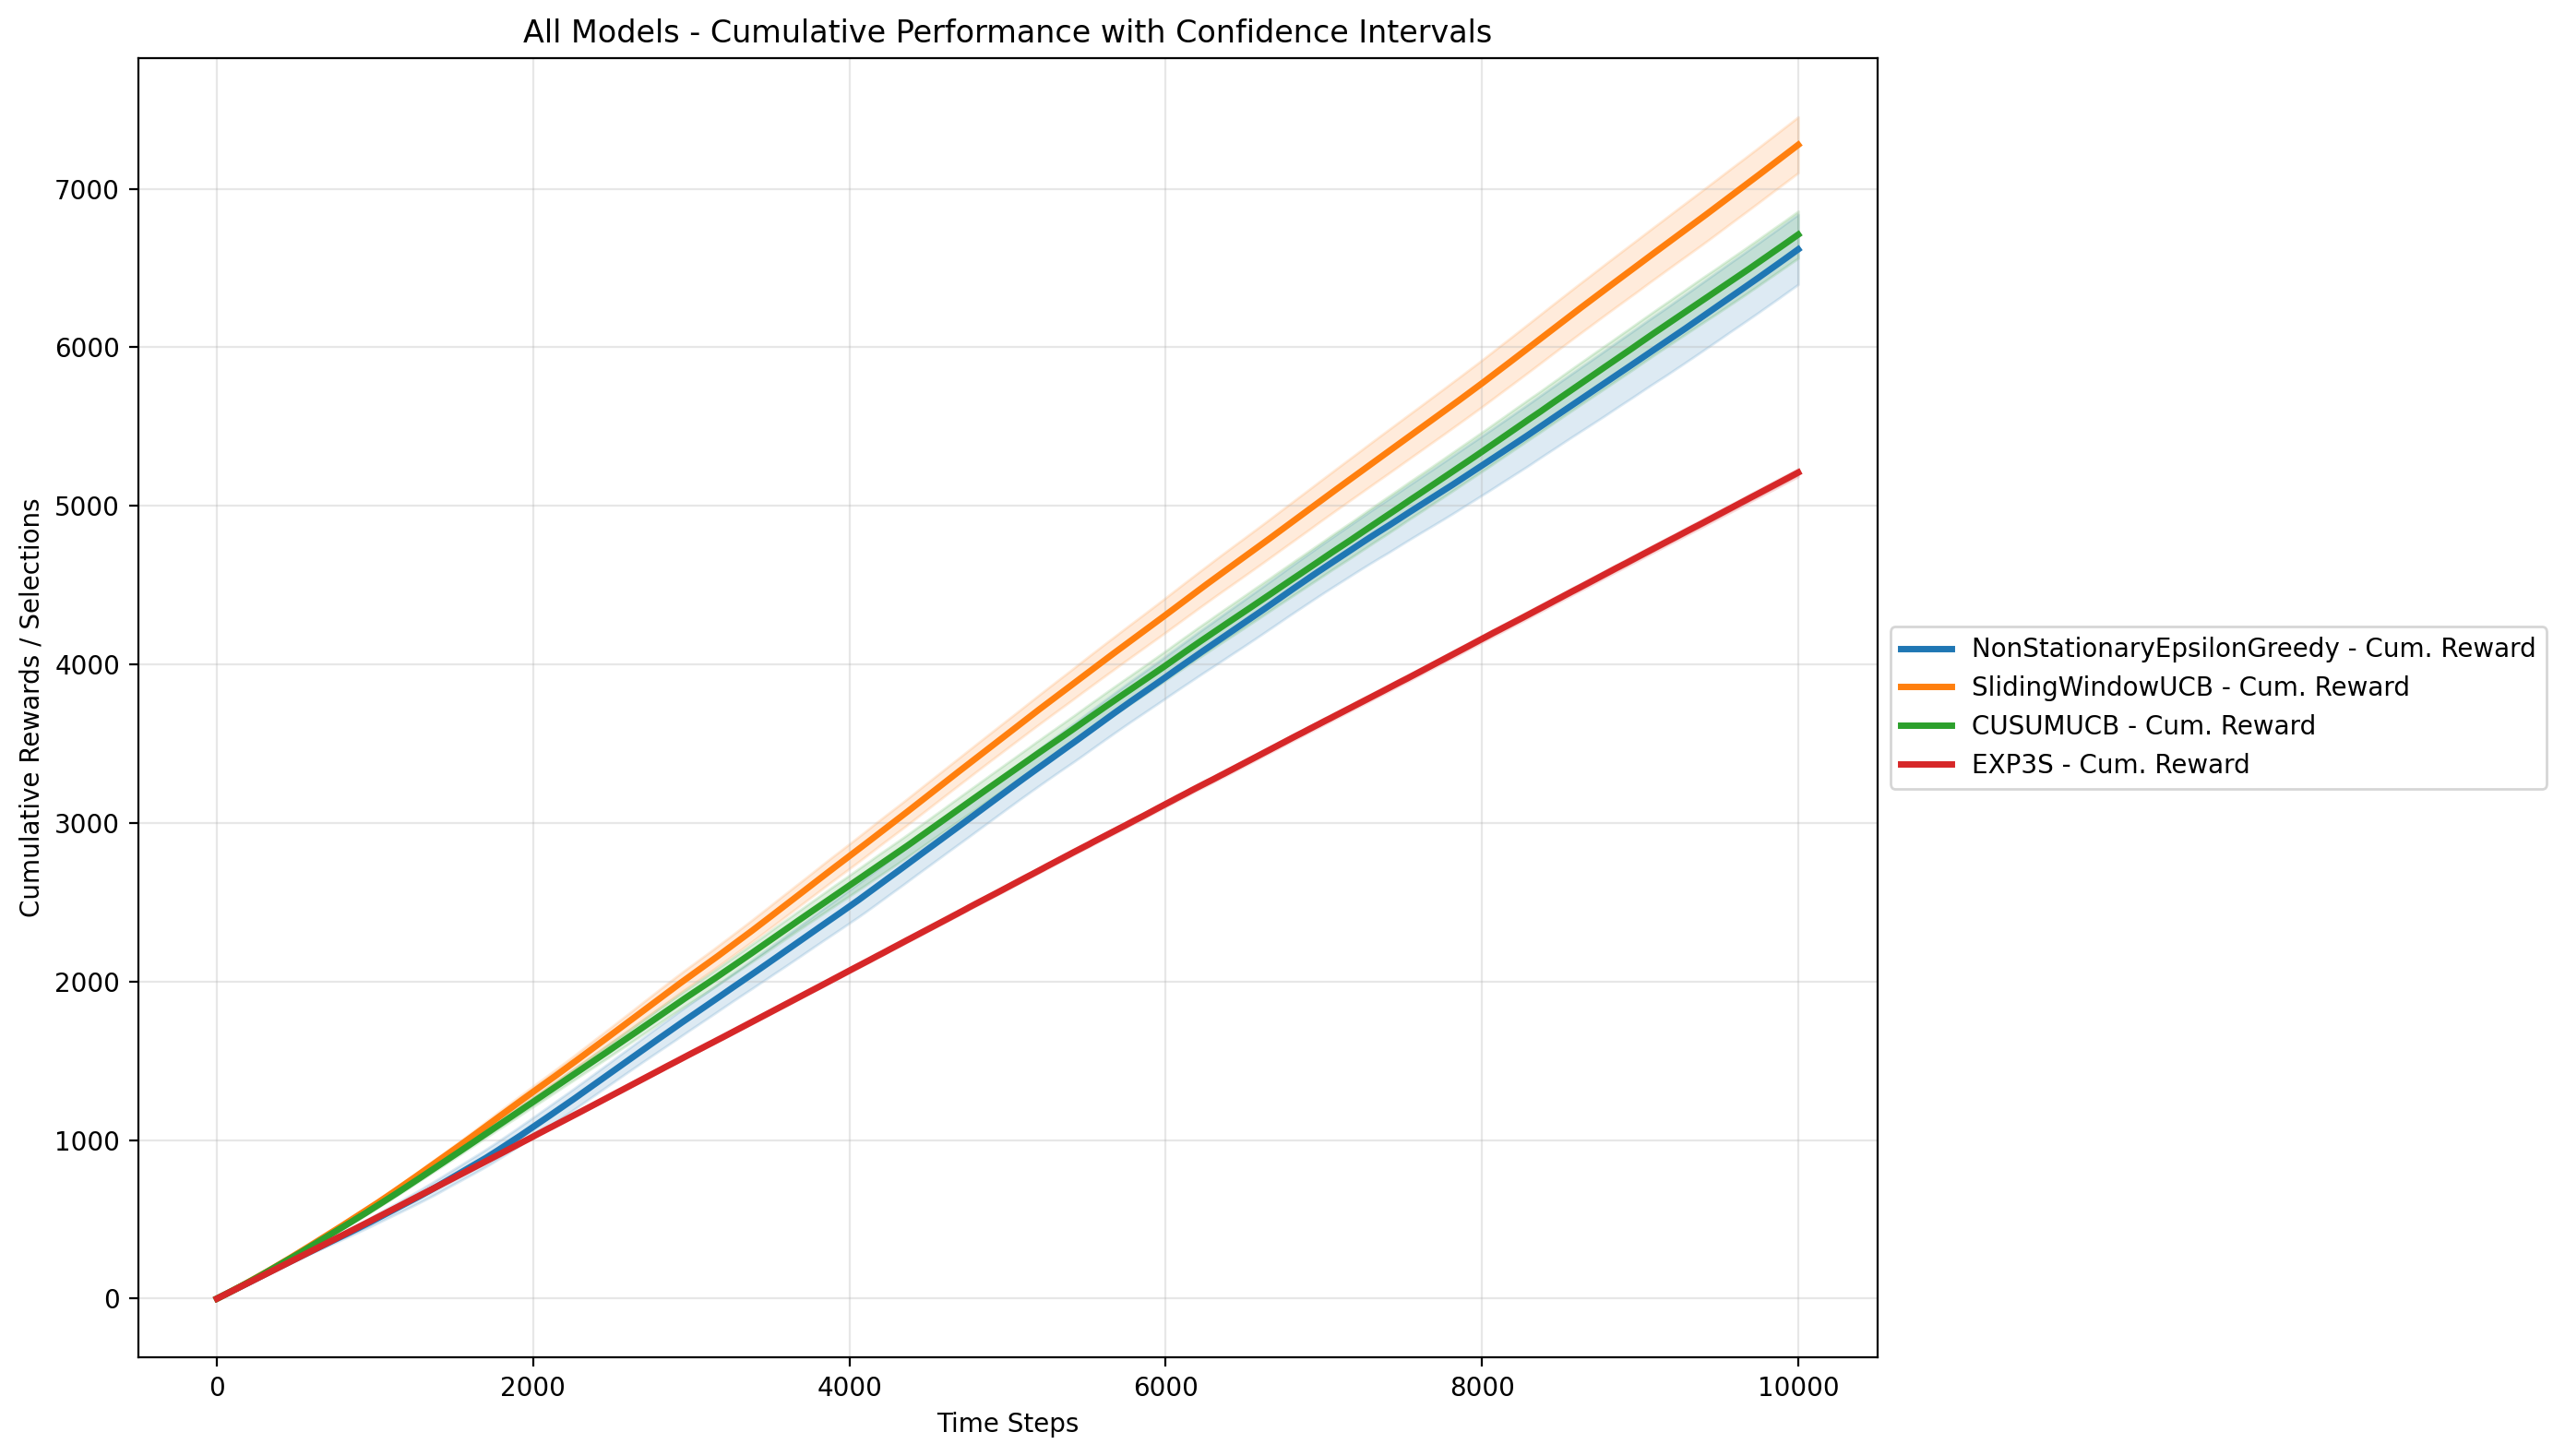
\includegraphics[width=0.9\linewidth]{model_cumulative_all_ci.png}
	\caption{Mean rolling average reward (top) and mean cumulative reward
	(bottom) for all algorithms over 10{,}000 steps, averaged over 50 runs with
	95\% confidence intervals.}
	\label{fig:models-perf}
\end{figure}

From these graphs we observe that Sliding-Window UCB is the clear winner in
terms of both adaptation speed and total reward. Its finite window allows it
to forget obsolete rewards and focus on the most recent regime. CUSUM-UCB
performs similarly but with occasional dips corresponding to detected changes
and subsequent restarts. The Non-Stationary $\varepsilon$-Greedy baseline
eventually tracks the better arm but does so more slowly because its constant
step-size must trade off reactivity against variance.

EXP3.S, designed for adversarial bandits, behaves conservatively in this
stochastic drift scenario. By updating only the weight of the played arm using
an importance-weighted estimate and mixing with uniform exploration, EXP3.S
obtains strong worst-case guarantees but fails to fully exploit the structure
of the drifting user. This leads to consistently lower average and cumulative
rewards.

% ----------------------------------------------------
\section{Discussion}

The main challenge in this project was to disentangle algorithmic behavior
from environmental effects. Synthetic drift parameters, horizon length, and
hyperparameters all influence performance. By fixing a simple two-arm setting
and running many seeds, we were able to uncover consistent patterns: methods
that explicitly forget or reset old information adapt best to user drift.

Compared to related work, our implementation of SW-UCB and CUSUM-UCB confirms
their advantage in non-stationary stochastic environments. Our experiments also
highlight a common misconception: adversarial bandit algorithms such as
EXP3.S, while theoretically appealing, are not necessarily competitive in
smoothly drifting recommender scenarios where rewards are still generated from
underlying distributions. For practitioners, this suggests prioritizing
sliding-window or change-detection schemes before moving to adversarial
methods.

% ----------------------------------------------------
\section{Conclusion}

This report presented a drifting-user simulator and a comparative study of four
adaptive bandit algorithms. In our synthetic non-stationary environment,
Sliding-Window UCB consistently achieved the highest long-run reward, followed
by CUSUM-UCB and Non-Stationary $\varepsilon$-Greedy, with EXP3.S lagging
behind. These results support the use of explicit forgetting mechanisms for
recommender systems facing gradual preference drift.

Future extensions include richer context features, multiple users, more complex
drift patterns, and offline evaluation on logged interaction data. A systematic
hyperparameter study would also clarify how robust the observed ranking is
across environments and design choices.

\bibliographystyle{IEEEtran}
\bibliography{references}

\end{document}
